\documentclass[conference]{IEEEtran}
\usepackage{blindtext, graphicx}

\usepackage[slovak]{babel}
\usepackage[utf8]{inputenc}
\usepackage{cite}

\usepackage{url}
\usepackage{amsmath}

\usepackage{algorithm}
\usepackage{algpseudocode}

\algnewcommand\algorithmicforeach{\textbf{for each}}
\algdef{S}[FOR]{ForEach}[1]{\algorithmicforeach\ #1\ \algorithmicdo}

% correct bad hyphenation here
\hyphenation{op-tical net-works semi-conduc-tor}

\begin{document}
%
% paper title
% can use linebreaks \\ within to get better formatting as desired
\title{Implementácia modifikovaného algoritmu SHA-1 v jazyku C (CPU) a CUDA (GPU)}

% author names and affiliations
% use a multiple column layout for up to three different
% affiliations
\author{\IEEEauthorblockN{Peter Kaňuch}
\IEEEauthorblockA{Fakulta informatiky a informačných technológií\\
Slovenská Technická Univerzita\\
Slovenská republika, 841 04 Bratislava IV\\
Email: xkanuch@stuba.sk}}

% use for special paper notices
%\IEEEspecialpapernotice{(Invited Paper)}

% make the title area
\maketitle

\begin{abstract}
%\boldmath
Keďže grafické procesory sú prispôsobené pre paralelné spracovanie úloh na viacerých jadrách, implementácia takto prispôsobeného problému zníži čas potrebný na jeho vykonanie oproti klasickým počítačovým procesorom. V článku sa zaoberáme základnou architektúrou CPU a GPU procesorov, implementáciou hashovacieho algoritmu SHA-1 upraveného pre paralelné spracovanie uvedeného v článku \cite{MSHA}, s cieľom poukázať na hlavné rozdiely v architektúrach týchto procesorov. Našim hlavným cieľom je však ukázať, prečo v súčasnosti neexistuje automatický paralelizmus výpočtovo náročných úloh a ich vykonávanie na grafických procesoroch.
\end{abstract}

\begin{IEEEkeywords}
SHA-1, Modified SHA-1, CPU architecture, GPU architecture, Automatic parallelism for GPU 
\end{IEEEkeywords}

\IEEEpeerreviewmaketitle

\section{Úvod}

V posledných rokoch sa grafické procesory začali dostávať do popredia, nie len na spracovanie obrazu, ale aj na vykonávanie, či spracovanie rôznych náročných výpočtových úloch. Architektúra grafických procesorov bola navrhnutá a optimalizovaná pre paralelné spracovanie inštrukcií a dát, zatiaľ čo CPU sú optimalizované pre rýchle sequenčné spracovanie toku programu. \\
Zvyšovanie rýchlosti a výpočtovej výkonnosti počítačov je čoraz viac žiadanejšie. Na rôzne výpočtovo náročné úlohy sa používajú multipočítače, no aj pre tieto výkonné stroje by niektoré úlohy trvali dlho. Preto sa vymýšľajú rôzne spôsoby, ako dosiahnúť lepší výkon. Jedným zo spôsobou je preniesť spracovanie náročných úloh na grafické procesory. To si však vyžaduje určité technické znalosti. V tomto článku preto porovnáme základnú architektúru CPU a GPU. Vysvetlíme princíp fungovania algoritmu SHA-1 a jeho modifikovanej paralelizovanej verzii, pretože hashovacie funkcie sú používané v oblasti počítačovej bezpečnosti. Daný algoritmus implementujeme v programovacom jazyku C pre klasické a v jazyku CUDA pre grafické procesory. Výsledky ukazujú porovnanie nameraných časov vykonávania daného algoritmu na CPU a GPU. Taktiež daný algoritmus porovnávame s implementáciou štandartne používaného nástroja pre výpočet hashovacích funkcií SHA. V závere diskutujeme, prečo ešte v súčasnosti neexistuje automatický paralelizmus a automatické vykonávanie výpočtovo náročných úloch na grafických procesoroch.

\section{CPU verzus GPU architektúra}

Aj keď sa zdá, že grafické procesory by mohli svojou výkonnosťou nahradiť klasické počítačové procesory, nie je tomu tak. CPU boli navrhnuté pre dosiahnutie čo najlepšieho výkonu pre sequenčné spracovanie dát, grafické procesory boli navrhnuté za účelom paralelného vykonávania inštrukcií. Pri porovnaní týchto procesorov CPU majú/sú \cite{gpuRowe}:

\begin{enumerate}
	\item{menej výpočtových jednotiek}
	\item{optimalizované pre sériové operácie}
	\item{nízku toleranciu latencie}
	\item{podporu pre paralelné spracovanie (novšie verzie)}
\end{enumerate}

a GPU:

\begin{enumerate}
	\item{viac výpočtových jednotiek}
	\item{vstavané pre paralelné operácie}
	\item{vysokú toleranciu latencie}
	\item{vysokú priepustnosť}
	\item{lepšiu logiku riadenia}
\end{enumerate}


\begin{figure}[!h]
\centering
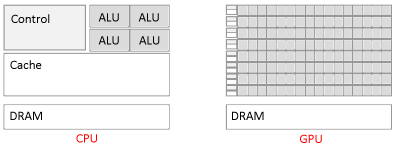
\includegraphics[width=2.5in]{img/CPU-GPU-3}
\caption{CPU vz. GPU}
\end{figure}


\subsection{Architektúra počítačových procesorov}

CPU (Central Processing Unit) alebo aj procesor, je hlavný komponent počítača, ktorý načítava, spracováva a vykonáva inštrukcie nad rôznymi dátami. Procesor pozostáva z dvoch hlavných častí:

\begin{itemize}
	\item{kontrolná jednotka (CU)}
	\item{aritmeticko-logická jednotka (ALU)}
\end{itemize}

Základný procesor pozostáva z piatich fáz \cite{hennessy2007compute}: 

\begin{itemize}
	\item{IF (Instruction Fetch) - fáza, v ktorej sa načítava inštrukcia z pamäte do procesora na základe adresy v registry IP/PC (instruction pointer/program counter) a jeho následnej inkrementácii na ďalšiu adresu }
	\item{ID (Instruction Decode) - zabezpečuje dekódovanie inštrukcie}
	\item{EX (Execute) - fáza, v ktorej procesor vykonáva rôzne výpočty pomocou ALU}
	\item{MEM (Memory Access) - v tejto fáze, procesor pristupuje do pamäte pre načítanie alebo uloženie dát}
	\item{WB (Write Back) - procesor zapíše výsledky(hodnoty z predošlých fáz vypočítané v ALU) alebo hodnoty načítané z pamäte v predchádzajúcej fáze do registrov}
\end{itemize}

\begin{figure}[!h]
\centering
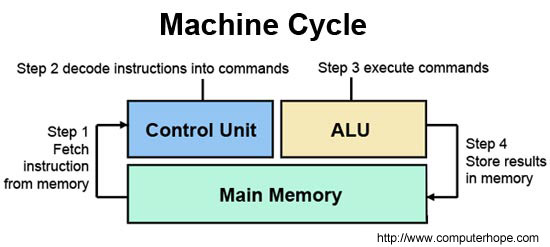
\includegraphics[width=3.5in]{img/CPU-cycle}
\caption{Základný cyklus procesora}
\end{figure}

Takáto základná architektúra bola postupne vylepšovaná rôznymi mechanizmami (prúdovým spracovaním, detekciou a riešením hazardov, či závislostí, predikciou vetvenia a iné) pre dosiahnutie čo najlepšieho výkonu, t.j. dosiahnutie čo najmenšieho CPI (CPI - počet cyklov na inštrukciu).

Jedným z vylepšení procesora je \textit{prúdové spracovanie.} To spočíva v tom, že v každom hodinovom cykle procesora dokážeme začať spracovávať novú inštrukciu \cite{hennessy2007compute}. Tým dokážeme znížiť vykonávanie jednej inštrukcie z piatich cyklov  na hodnotu blízkej jedna. Nie je to však jednoduché. Vznikajú takzvané \textit{hazardy} a \textit{závislosti v programe}. 

Ďalším vylepšením procesora, kedy inžinieri chceli zvýšiť výkonnosť procesora, bolo vymyslením \textit{Hyper-threading}-u. Hyper-threading vytvára z jedného fyzického, viacero logických procesorov \cite{hyperthreading}. Procesor podporujúci danú technológiu si dokáže zapamätať viacero stavov procesora pomocou pridanej kompletnej sady jednotlivých registrov (základných, kontrolných, ...).  
Princíp fungovania je jednoduchý: V každom čase sa spracováva len jedna úloha. Procesor však dokáže veľmi rýchlo prepínať medzi jednotlivými úlohami, čo vytvára pocit, že bežia súčasne. \newline
Základnou nevýhodou hyper-threading-u je, že ostatné súčasti procesora (ALU, MMU, FPU, SIMD) zdieľa medzi úlohami (viď obr. \ref{img} \cite{picture}) \cite{hyper2}. Preto tento spôsob zlepšenia nám nezvýši výkon pri výpočtovo náročných úlohách (napr. násobenie matíc).

\begin{figure}[!h]
\centering
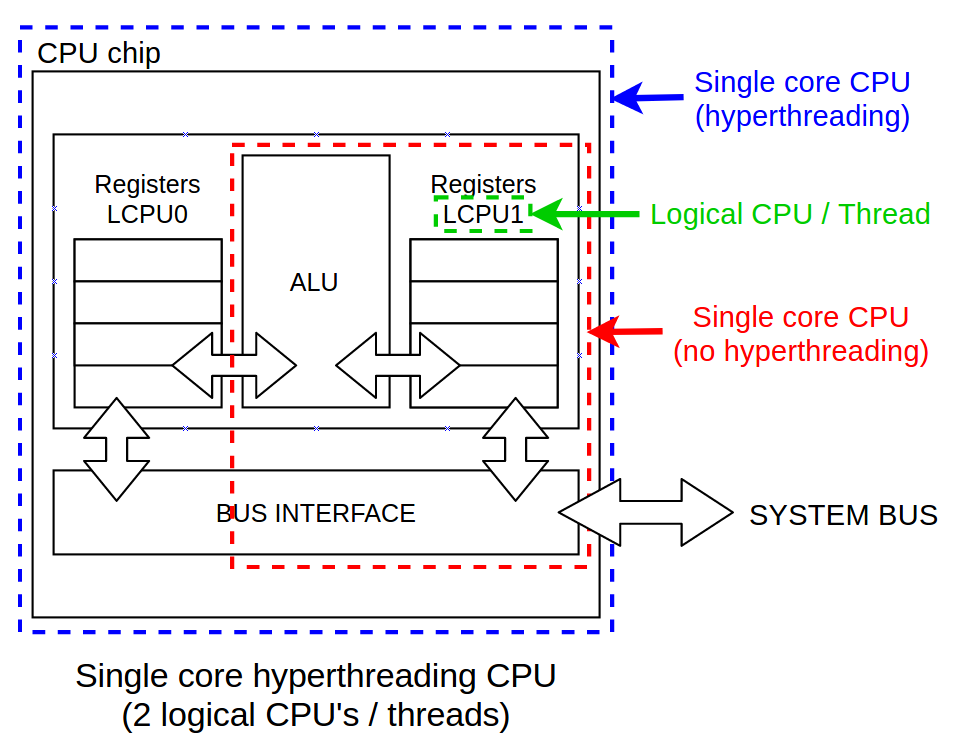
\includegraphics[width=2.75in]{img/hyper}
\caption{1-jadrový procesor s hyper-threading \label{img}}
\end{figure}

Iným vylepšením procesora je pridanie viacerých jadier procesora na jeden spoločný čip (viď obr. \ref{quad}\cite{picture}). Týmto spôsobom sa nám znásobi aj počet vykonávacich jednotiek 
čím dosiahneme aj znásobenie výpočtového výkonu. Súčasné bežné procesory v prenosných počítačoch obsahujú dve až štyri jadrá. Najvýkonnejšie procesory pozostávajú zo šiestich a viac jadier (12 až 18).  

\begin{figure}[!h]
\centering
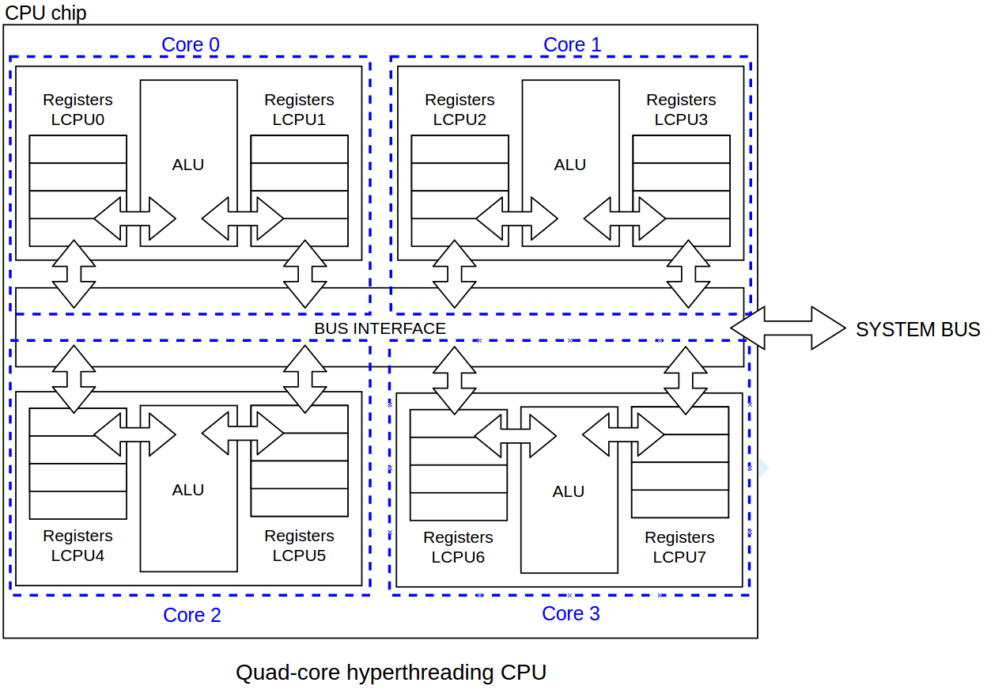
\includegraphics[width=3in]{img/quad}
\caption{4-jadrový procesor s hyper-threading \label{quad}}
\end{figure}

\subsection{Architektúra grafických procesorov}

Grafické procesory sú navrhnuté tak, aby čo najrýchlesjšie dokázali vykonať paralelizovateľný kód. Napríklad vykonať rovnaké inštrukcie nad rôznymi dátami. Do návrhu boli zahrnuté 3 myšlienky \cite{GPU2011Fatahalian}: 

\begin{enumerate}
	\item{Pre GPU odstrániť tie časti CPU, ktoré umožňujú rýchle sequenčné výkonávanie inštrukcií.}\\
	\item{Znížiť náročnosť riadenia inštrukcií vo viacerých ALU.}\\
	\item{Predchádzať hazardom pomocou začatia vykonávania iného bloku.}
\end{enumerate}

\begin{figure}[!h]
\centering
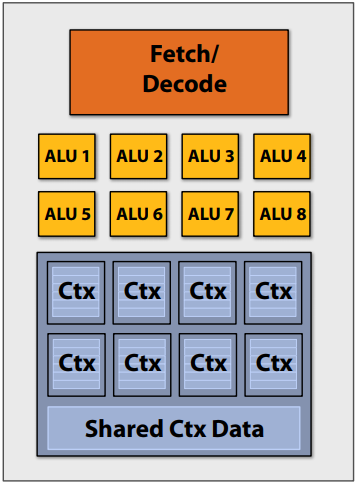
\includegraphics[width=2.1in]{img/GPU-core}
\caption{Jedno jadro grafického procesora \label{core}}
\end{figure}

Grafický procesor pozostáva z nasledujúcich častí \cite{tatourian}:

\begin{enumerate}
	\item{Globálna pamäť}
	\item{Multi-procesor - ten sa skladá z:}
	\begin{itemize}
		\item{Kontrolné jednotky}
		\item{Registre}
		\item{Výkonné jednotky}
		\item{Cache pamäte}
	\end{itemize}
\end{enumerate}

Programy, napísané pre grafické procesory, nevedia pristupovať k dátam uloženým v hlavnej pamäti \cite{gpuRowe}. Taktiež, GPU boli navrhnuté pre rýchle paralelné spracovanie dát a nepodporujú niektoré funkcie operačného systému. Z tohto dôvodu musia CPU a GPU procesory spolupracovať. Za vykonanie programu na grafike je zodpovedný CPU \cite{tatourian}. Ten má za úlohu:

\begin{itemize}
	\item{Prekopírovať dáta potrebné pre vykonanie programu z hlavnej pamäte do video pamäte.}
	\item{Vložiť program (GPU kernel) naprogramovaný programátorom na grafický procesor.}
	\item{Po dokončení a spracovaní dát nakopírovať späť výsledné dáta z video pamäte do hlavnej pamäte}
\end{itemize}

\begin{figure}[!h]
\centering
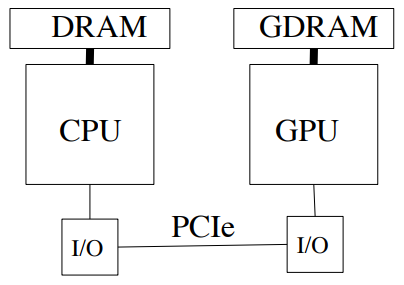
\includegraphics[width=1.5in]{img/CPU+GPU}
\caption{Spojenie CPU a GPU}
\end{figure}

%**********************************************************************************************************************
\section{Opis riešenia}

Pre porovnanie časov vykonávania programu na CPU a GPU, sme sa rozhodli naprogramovať algoritmus SHA-1 v jazyku C pre CPU a v jazyku CUDA pre grafické procesory. Klasický algoritmus SHA však nie je paralelizovateľný, a preto sme implementovali jednu z jeho modifikácií pre paralelné spracovanie. Výber problému nie je veľmi vhodný vzhľadom na porovnanie architektúry procesorov, keďže daný problém nepozostáva zo zložitých aritmeticko-logických operácií.

\subsection{Algoritmus SHA-1 a jeho modifikácia}

Všeobecný algoritmus SHA pozostáva z nasledujúcich krokov:

\begin{enumerate}
	\item{Predspracovanie}
	\begin{itemize}
		\item{Zarovnanie správy}
		\item{Rozdelenie na bloky}
		\item{Nastavenie počiatočného výsledku hash-u}\\
	\end{itemize}
	\item{Výpočet hash-u}
\end{enumerate}

Princíp fungovania SHA: 
\begin{enumerate}
	\item{Zarovnanie správy pomocou nulových bajtov a doplnením veľkosti správy na koniec}
	\item{Rozdelenie správy na bloky o veľkosti 64 bajtov}
	\item{Nastavenie počiatočného výsledku hash-u}
	\item{Vykonanie operácií a pripojenie medzivýsledku ku finálnemu hashu pre každý blok}
\end{enumerate}

\begin{algorithm}
   \caption{SHA-1 \cite{sha-algo}}
    \begin{algorithmic}[1]
      \Function{SHA}{$Message$ $M$}

        \State padding(M) \Comment{Put zero bytes into message and its size at the end}
        \State  Set ${H_0}$ \Comment{Initial value of hash}
     	\ForEach {$block \in \mathcal M $} \Comment{512 bit block size}
     		\For{$i = 0$ to $15$}
     			\State $W_i = M_i$
     		\EndFor
     		\For{$i = 16$ to $79$}
     			\State $W_i = ROTL^1(W_{i-3} \oplus W_{i-8} \oplus W_{i-14} \oplus W_{i-16})$
     		\EndFor
		\State Set ${a, b \ldots e}$ with ${H_{0..4}^{i-1}}$
		\For{$i = 0$ to $79$} \Comment{f = Ch for i == 0 ... 19; Parity for i == 20 ... 39 \& 60 ... 79; Maj for i == 40...59}
			\State  $T = ROTL^5(a) + f(b,c,d) + e + K_i + W_i)$
			\State  $e = d$
			\State  $d = c$
			\State  $c = ROTL^{30}(b)$
			\State  $b = a$
			\State  $a = T$
     		\EndFor		
     	\EndFor
   	\State ${H_{0..4}^{i-1}}$ = ${a, b \ldots e}$ + ${H_{0..4}^{i-1}}$
       \EndFunction
\end{algorithmic}
\end{algorithm}


\begin{figure}[!h]
\centering
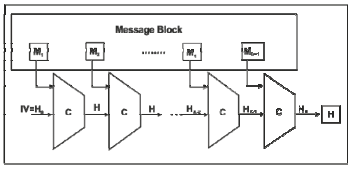
\includegraphics[width=3in]{img/SHA}
\caption{Grafické znázornenie klasického algoritmu SHA}
\end{figure}

Princíp fungovania modifikovanej SHA: 
\begin{enumerate}
	\item{Rozdelenie správy na bloky o veľkosti 64 bajtov}
	\item{Pre každý blok}
	\begin{enumerate}
		\item{Nastavenie počiatočnej hodnoty}
		\item{Vykonanie operácií}
		\item{Pripojenie výsledku k počiatočnej hodnote}
	\end{enumerate}
	\item{Spojenie výsledkov jednotlivých blokov}
	\item{Ak veľkosť bloku nerovná sa 20 bajtov $\implies$ pokračuj v bode 1.}
\end{enumerate}


\begin{algorithm}
   \caption{Modified SHA-1 (pseudo code) \cite{MSHA}}
    \begin{algorithmic}[1]
      \Function{MSHA}{$Message$ $M$}

        \State ${padding(M)}$ \Comment{Put zero bytes into message and its size at the end}
        \State ${Blocks(M)}$ \Comment{Breaking message into 64 bytes blocks}
	\ForEach {$block \in \mathcal M $} \Comment{Each block is independent}
     		\State ${H_i = SHA(block)}$		
     	\EndFor
   	\State ${H += H_i}$ \Comment{+ mean concatenate}   	
   	\If {(size(H) != 20B)} ${MSHA(H)}$
   		\Else {  return}
   	\EndIf
       \EndFunction
\end{algorithmic}
\end{algorithm}


\begin{figure}[!h]
\centering
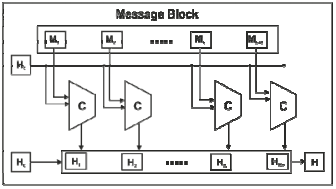
\includegraphics[width=3in]{img/MSHA}
\caption{Grafické znázornenie modifikovaného algoritmu SHA}
\end{figure}


\subsection{Vlastnosti SHA-1 a jeho modifikovanej verzie}

Pre všetky hashovacie funkcie je dôležité spĺňať nasledujúce vlastnosti \cite{CHF}:

\begin{itemize}
	\item{Ireverzibilnosť hashu (Preimage resistance) - pre daný hash je ťažké nájsť správu, po ktorej zahashovaní dostaneme pôvodný hash}
	\item{Odolnosť voči kolíziám - je ťažké nájsť také dve rôzne správy, ktorých výsledky hashu sa rovnajú}
\end{itemize}

Daný modifikovaný algoritmus SHA-1 by mal spĺňať všetky vlastnosti hashovacích funkcií, viď článok\cite{MSHA}.

\subsection{Testovacie prostredie}

Dané navrhnuté riešenie implementácie modifikovaného algoritmu SHA-1 bolo realizované na nasledujúcom technickom vybavení počítača (Hardware):

\begin{itemize}
	\item{Procesor: Intel Core i3-4100M 2.50GHz, 2 Core(s), 4 Logical Processor(s)}
	\item{Hlavná pamäť (RAM): 12.0 GB DDR3, 2.5GHz}
	\item{Grafický procesor: NVIDIA GeForce GT 740M, 2.0 GB DDR3}
\end{itemize}

a programového vybavenia:

\begin{itemize}
	\item{Operačný systém: Windows 8.1 - 64-bit}
	\item{Vývojové prostredie:}
	\begin{itemize}
		\item{Microsoft Visual Studio Enterprise 2015 v14.0.25431.01}
		\item{Nsight Visual Studio Edition v5.4}
	\end{itemize}
\end{itemize}

\subsection{Implementácia}

Vyššie opísaný modifikovaný algoritmus SHA-1 sme implementovali v jazyku C a v jazyku CUDA. Pre porovnanie výpočtového výkonu daných procesorov sme sa rozhodli merať čas len funkcie, ktorá priamo vykonáva daný výpočet hashu. Čas potrebný na prenos dát z hlavnej pamäte do video pamäte a späť a čas potrebný pre načítanie súboru do pamäte sme nezáratavali do celkového času z dôvodu, že pri daných časoch by sme už neporovnávali samotný výkon procesorov, čo bolo našou úlohou.\\
Implementácia na CPU vyzerá rovnako ako opísaný algoritmus pomocou pseudo kódu vyššie v článku. Implementácia v jazyku CUDA pre grafické procesory je trochu odlišná. Rozdelenie správy do jednotlivých blokov je zabezpečené pomocou indexovania na grafickej karte.

\begin{algorithm}
   \caption{Modified SHA-1 (pseudo code CUDA)}
    \begin{algorithmic}[1]
      \Function{cuda}{$Message$ $M$}
        	\State ${padding(M)}$ \Comment{Put zero bytes into message and its size at the end}
        	\State ${copyToDevice(M)}$ \Comment{Copy message to video RAM}
     	\State ${SHA<<< blocks, 512 >>> (m);}$ \Comment{blocks - number of message blocks, 1 block = 1 core GPU, 512 - number of threads for 1 block}
     	\State ${H = copyToHost()}$ \Comment{Copy result to host from video RAM}	
   	
   	\If {(size(H) != 20B)} ${cuda(H)}$
   		\Else {  return}
   	\EndIf
       \EndFunction
\end{algorithmic}
\end{algorithm}

Meranie času na CPU bolo realizované pomocou knižnice ${<sys\backslash timeb.h>}$ a v jazyku CUDA sme použili ${cudaEvent}$ funckie cudaEventRecord() pre časové pečiatky vykonávania na GPU a cudaEventElapsedTime() pre vypočítanie rozdielu časov. 


\section{Výsledky a grafické porovnanie}

\subsection{Provonanie implementácií}
Dané implementácie sme navzájom porovnali na vzorke rôznych veľkosti súborov od 0,250MB až po 600MB. Dané merania pre každú veľkosť súboru sme uskutočnili 10 krát pre obe implementácie. Následne sme vypočítali priemer z meraní a zrýchlenie medzi CPU a GPU. 

\begin{figure}[h!]
\centering
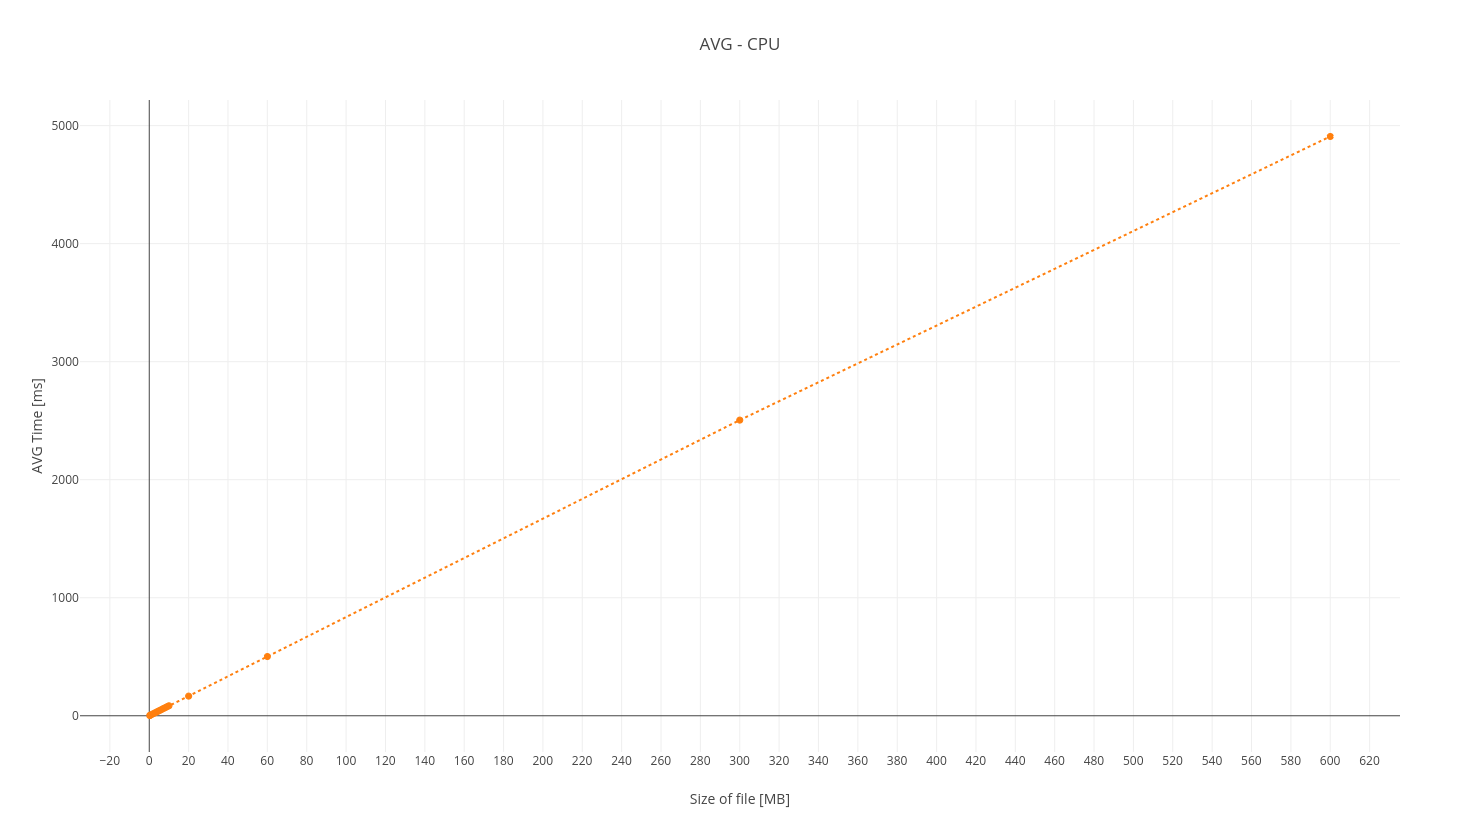
\includegraphics[width=3in]{img/AVG-CPU-new}
\caption{Priemerný čas výpočtu MSHA-1 na CPU}
\end{figure}

\begin{figure}[h!]
\centering
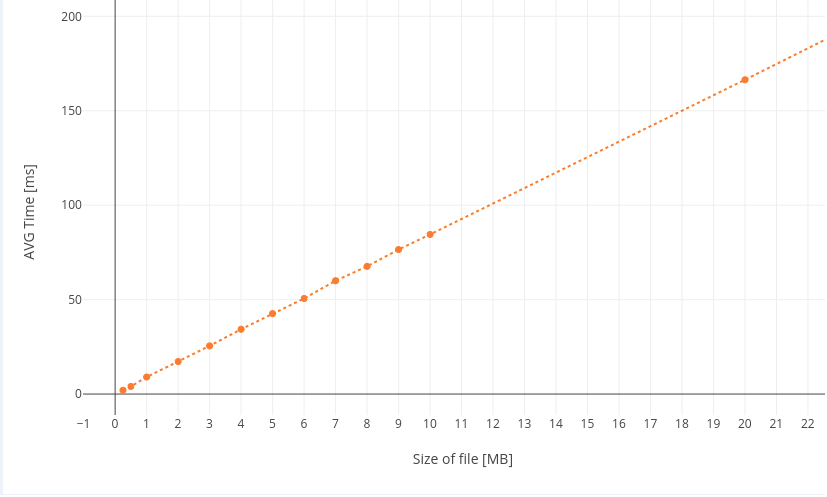
\includegraphics[width=3in]{img/AVG-CPU-new2}
\caption{Priemerný čas výpočtu MSHA-1 na CPU  (detailnejšie zobrazenie)}
\end{figure}


\begin{figure}[h!]
\centering
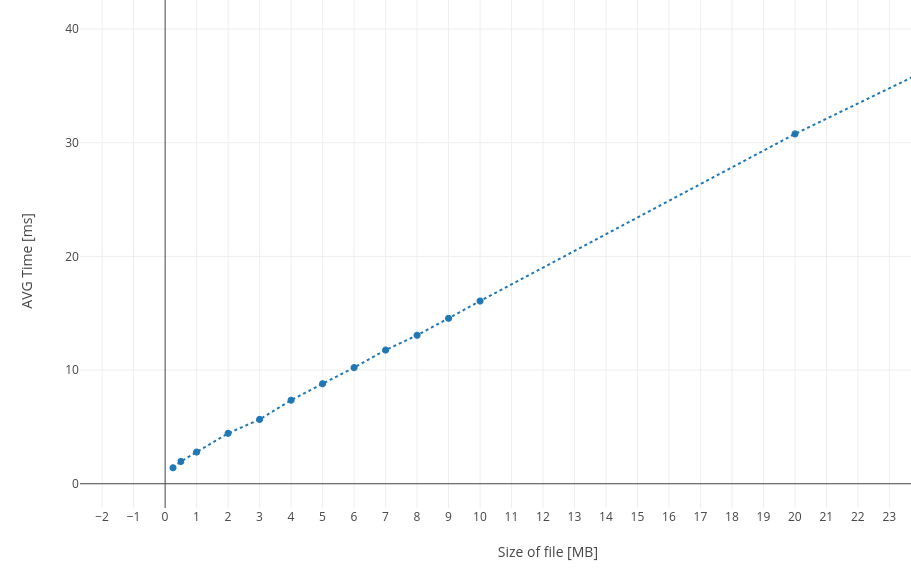
\includegraphics[width=3in]{img/AVG-GPU-new3}
\caption{Priemerný čas výpočtu MSHA-1 na GPU (detailnejšie zobrazenie)}
\end{figure}

\begin{figure}[h!]
\centering
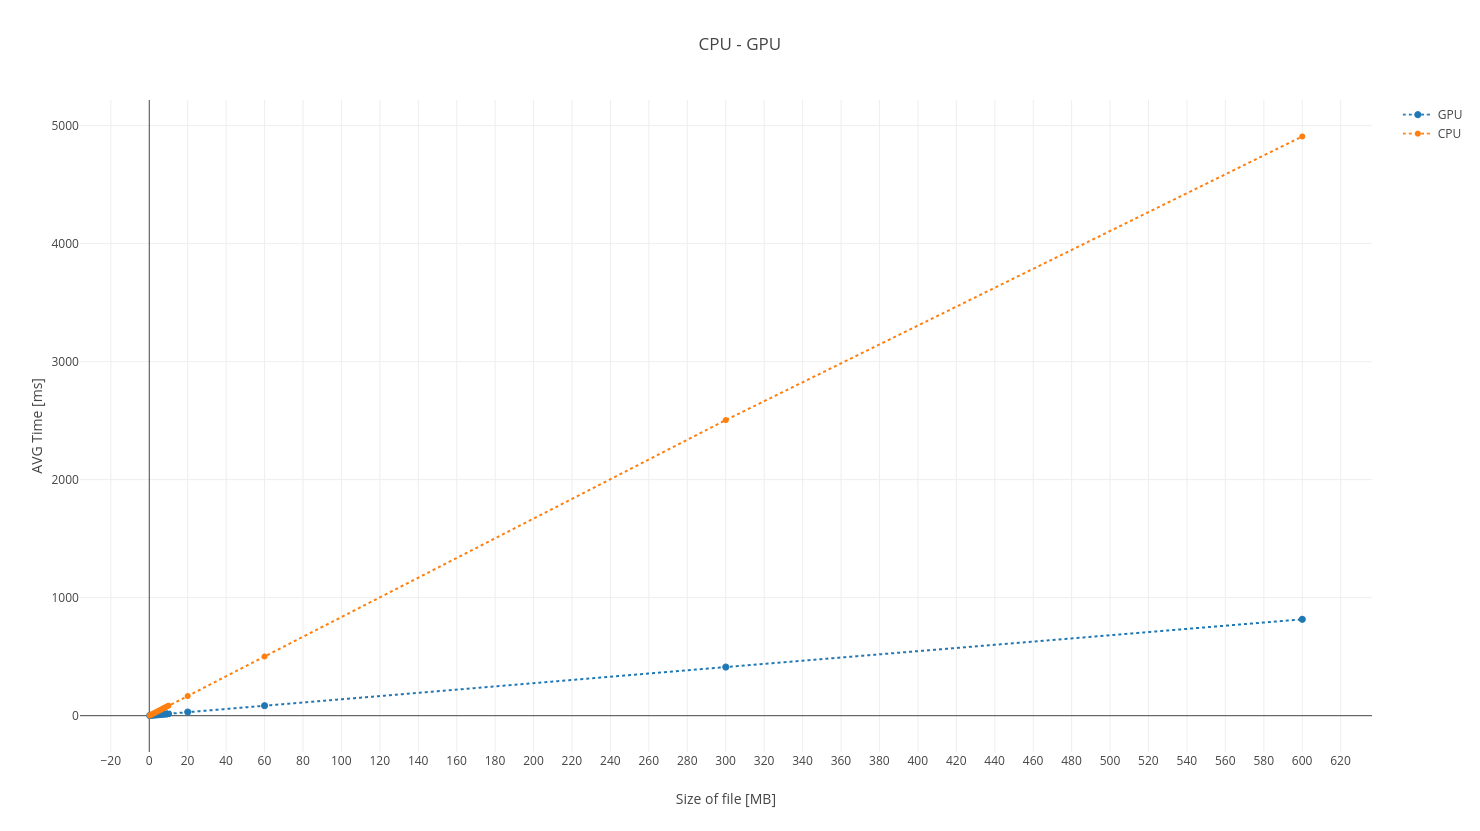
\includegraphics[width=3in]{img/CPU-GPU-new}
\caption{Porovnanie CPU a GPU časov pre jednotlivé veľkosti súborov}
\end{figure}

\begin{figure}[h!]
\centering
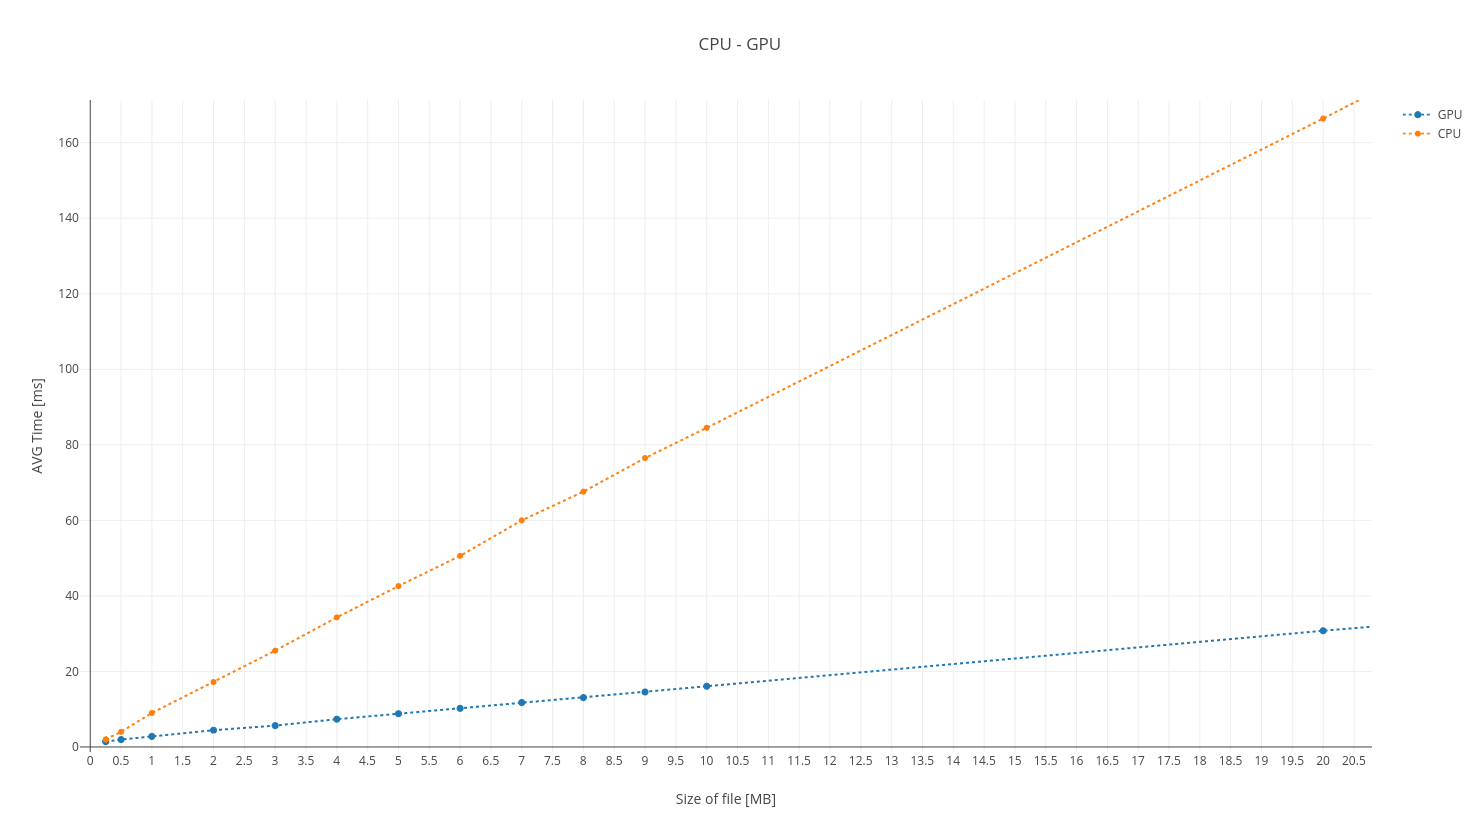
\includegraphics[width=3in]{img/CPU-GPU-new2}
\caption{Porovnanie CPU a GPU časov pre jednotlivé veľkosti súborov (detailnejšie zobrazenie)}
\end{figure}

\begin{figure}[h!]
\centering
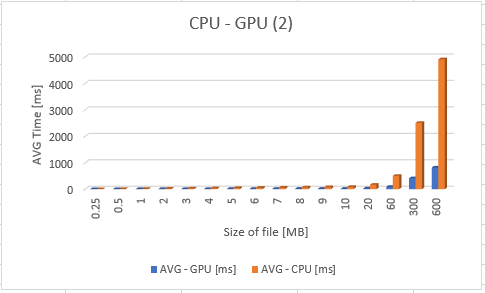
\includegraphics[width=3in]{img/CPU-GPU2}
\caption{Porovnanie CPU a GPU časov pre jednotlivé veľkosti súborov}
\end{figure}

\begin{figure}[h!]
\centering
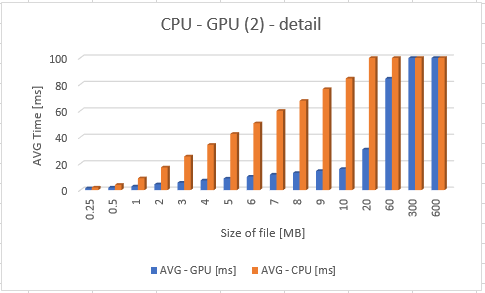
\includegraphics[width=3in]{img/CPU-GPUdetail2}
\caption{Porovnanie CPU a GPU časov pre jednotlivé veľkosti súborov (detailnejšie zobrazenie)}
\end{figure}


\subsection{Porovnanie implementácie s reálnym nástrojom}

Implementáciu sme taktiež porovnali s reálnym nástrojom \textit{sha1sum}, používaným na hashovanie súborov, dostupným pre platformy Windows aj Linux. Do takéhoto porovnania sme započítali aj časy pre načítavanie súboru do pamäte. Nezarátavali sme však čas potrebný na presun dát z hlavnej pamäte do video pamäte. Pre odmeranie vykonávania hashu nástrojom sha1sum sme použili štandartne dostupný nástroj \textit{time}. Dané merania sme taktiež vykonali na pre rôzne veľkosti ako v predchádzajúcom prípade. 

\begin{figure}[h!]
\centering
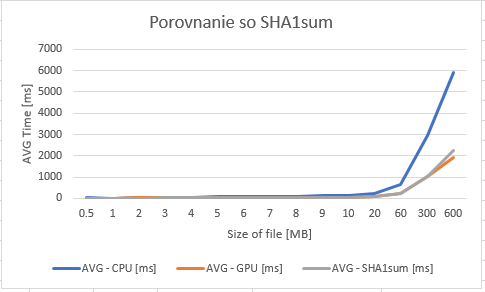
\includegraphics[width=3in]{img/sha1sum}
\caption{Porovnanie s nástrojom sha1sum}
\end{figure}

\begin{figure}[h!]
\centering
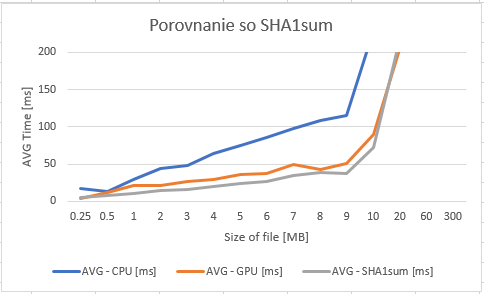
\includegraphics[width=3in]{img/sha1sumdetail}
\caption{Porovnanie s nástrojom sha1sum  (detailnejšie zobrazenie)}
\end{figure}


\section{Automatické využitie GPU}

Viacjadrové procesory spolu s kompilátormi v dnešnej dobe podporujú funkcionalitu pre automatický paralelizmus nie len na úrovni inštrukcií, ale aj jednoduchšie cykly v kóde \cite{automatic}. Pre zložitejšií zdrojový kód programu bolo vymyslené \textit{OpenMP}. To dokáže s minimálnym úsilím programátora vykonávať výpočtovo náročnú úlohu na viacerých jadrách procesora CPU.
Multijadrové procesory sa však ešte stále nevyrovnajú grafickým procesorom. Pre automatické paralelizované spracovanie na grafických procesoroch by kompilátor musel:

\begin{itemize}
	\item{nájsť nezávislé časti programu}
	\item{prekopírovať dáta z pamäte RAM do video pamäte a späť}
	\item{rozdeliť dáta pre jednotlivé bloky a thready GPU}
	\item{preložiť kód pre procesor GPU}
\end{itemize}

a zároveň by to muselo byť ovládané z CPU. Najnovšie grafické procesory však umožňujú spustiť väčší program (kernel), ktorý dokáže spúšťať menšie programy. To umožňuje spustenie bez potreby koordinácie CPU \cite{tatourian} a dosiahnutia tak vyššieho výkonu.

\section{Záver}
V článku sme porovnali implementáciu modifikovanej SHA-1 pre paralelné spracovanie na CPU a GPU, kde sme dosiahli určité zrýchlenie (viď tabuľka \ref{table}). Tieto implementácie sme taktiež porovnali aj s bežne používaným nástrojom sha1sum, kde naša implementácia algoritmu na CPU bola o čosi menej efektívna, čo odôvodňujeme optimalizáciou zdrojového kódu a trochu inou časovou náročnosťou klasickej a modifikovanej SHA-1. Implementáciou pre GPU sme sa však priblížili k hodnotám časov tohto nástroja. Môžme teda predpokladať, že pri použití zdrojového kódu z nástroja v našej implementácii na GPU, by sme zrýchlili výpočet hashu. 


\begin{table}[h!]
\centering
\caption{CPU vs. GPU}
\label{table}
\begin{tabular}{lllll}
Size {[}MB{]} & AVG - GPU {[}ms{]} & AVG - CPU {[}ms{]} & CPU/GPU     &  \\
0.25          & 1.4047648          & 2                  & 1.423725879 &  \\
0.5           & 1.958352           & 4                  & 2.042533722 &  \\
1             & 2.7868832          & 9                  & 3.229414135 &  \\
2             & 4.4332639          & 17.2               & 3.879760012 &  \\
3             & 5.6588672          & 25.5               & 4.506202231 &  \\
4             & 7.3489853          & 34.3               & 4.66731101  &  \\
5             & 8.7965731          & 42.6               & 4.842794974 &  \\
6             & 10.2195169         & 50.6               & 4.95131037  &  \\
7             & 11.7593665         & 60                 & 5.102315673 &  \\
8             & 13.0595455         & 67.6               & 5.1762904   &  \\
9             & 14.5545724         & 76.5               & 5.256080213 &  \\
10            & 16.0727678         & 84.5               & 5.257339685 &  \\
20            & 30.7733154         & 166.4              & 5.407282181 &  \\
60            & 84.3981097         & 501.7              & 5.944445933 &  \\
300           & 411.9776641        & 2504.7             & 6.079698533 & 
\end{tabular}
\end{table}


\begin{figure}[h!]
\centering
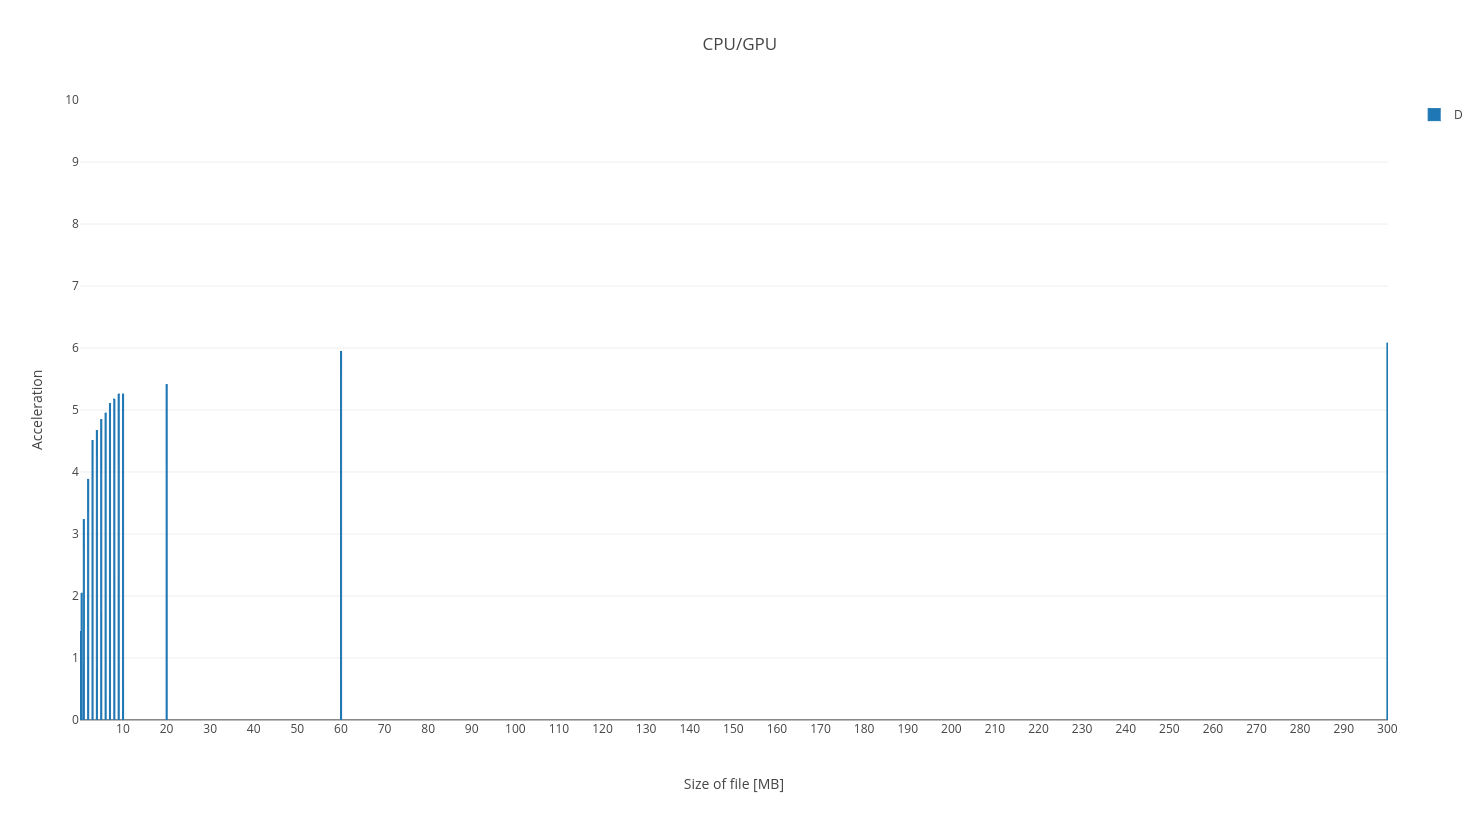
\includegraphics[width=3in]{img/acceleration}
\caption{Zobrazenie zrýchlenia implementácie medzi CPU a GPU}
\end{figure}






% Can use something like this to put references on a page
% by themselves when using endfloat and the captionsoff option.
\ifCLASSOPTIONcaptionsoff
  \newpage
\fi


\begin{thebibliography}{1}

\bibitem{hennessy2007compute}
HENNESSY, John L.; PATTERSON, David A. Computer architecture: a quantitative approach. Elsevier, 2007.

\bibitem{tatourian}
TATOURIAN, Alan. Nvidia gpu architecture and cuda programming environment. URL http://code. msdn. microsoft. com/windowsapps/NVIDIA-GPU-Architecture-45c11e6d, 2013.

\bibitem{hyperthreading}
PRECOMPUTATION, Speculative. Hyper-Threading Technology.

\bibitem{hyper2}Intel Pentium 4 3.06 GHz with Hyper-Threading support, \url{http://ixbtlabs.com/articles2/pentium43ghzht/}, Accessed: 12.11.2017.

\bibitem{GPU2011Fatahalian}How a GPU Works - Kayvon Fatahalian 15-462 (Fall 2011), \url{https://www.cs.cmu.edu/afs/cs/academic/class/15462-f11/www/lec_slides/lec19.pdf}, Accessed:12.11.2017.

\bibitem{picture}Differences between physical CPU vs logical CPU vs Core vs Thread vs Socket, \url{http://www.daniloaz.com/en/differences-between-physical-} \url{cpu-vs-logical-cpu-vs-core-vs-thread-vs-socket/}, Accessed: 12.11.2017.

\bibitem{gpuRowe}The Continuing Importance of GPUs For More Than Just Pretty Pictures - Jeff Rowe, \url{https://www10.mcadcafe.com/blogs/jeffrowe/2017/03/16/the-continuing-importance-of-gpus-for-more-than-just-pretty-pictures/}, Accessed:12.11.2017

\bibitem{sha-algo}GALLAGHER, Patrick; DIRECTOR, Acting. Secure hash standard (shs). FIPS PUB, 1995, 180-3.

\bibitem{CHF}ROGAWAY, Phillip; SHRIMPTON, Thomas. Cryptographic hash-function basics: Definitions, implications, and separations for preimage resistance, second-preimage resistance, and collision resistance. In: International Workshop on Fast Software Encryption. Springer, Berlin, Heidelberg, 2004. p. 371-388.

\bibitem{MSHA}KISHORE, Neha; KAPOOR, Bhanu. An efficient parallel algorithm for hash computation in security and forensics applications. In: Advance Computing Conference (IACC), 2014 IEEE International. IEEE, 2014. p. 873-877.

\bibitem{automatic}Automatic Parallelization with Intel® Compilers, Intel, November 2011, \url{https://software.intel.com/en-us/articles/automatic-parallelization-with-intel-compilers}, Accessed: 17.11.2017

\end{thebibliography}






\end{document}


